\documentclass[12pt]{article}

\usepackage{amsmath}
\usepackage{fancyvrb}
\usepackage{hyperref}
\usepackage{multicol}
\usepackage{wrapfig}
\usepackage{graphicx}
\graphicspath{ {./images/} }

\title{Insert Report Title Here}
\author{Benjamin White-Horne \\ \emph{Oxford University}}

\newcommand{\row}[1]{\texttt{#1}}
\newcommand{\br}[0]{\vspace{10pt} \noindent}
\newcommand{\footurl}[1]{\footnote{\url{#1}}}
\newcommand{\nth}[2]{#1\textsuperscript{#2}}

\begin{document}

\maketitle



\pagebreak

\tableofcontents



\pagebreak

\section{Abstract}

(Copied from my original report, and needs rewriting)

Change ringing is an artform which is almost exclusive to England, where people ring sets of bells
in continually evolving sequences, known as `changes' or `rows'.

More specifically, this project is concerned with the art of `composing' --- designing sequences of
rows for ringers to perform.  The art of composing predates computers by several centuries (the
ealiest surviving record of composing come from Fabian Stedman in the 1700s), so composers have
historically created compositions using pen, paper and copious amounts of both skill and patience.
However, change ringing compositions are at their core sequences of permutations and are therefore
extremely ameanable to both mathematical and computer analysis.  Even the first computers have been
used to mechanise parts of composing (namely `proving' --- verifying that a composition contains no
repeated rows), and as the increasing speed of computers has been exploited to allow computers to
fully generate some compositions.

But brute force is still no match for the creativity of human composers, and one mostly unexplored area
of composing is software that \emph{aids} human composers by giving instant feedback and
visualisations to a composer whilst not requiring them to make drastic changes to their workflow.
This is analogous to what software like Musescore or Sibelius do for composing music.



\pagebreak

\section{Overview of Change Ringing}

This project is to build a tool to help composers design complex sequences of ringing of church
bells.  Change ringing is a very niche and varied activity so this section will serve as a quick
introduction to the topic and overview of the aspects of change ringing which are most relevant to
this project.  A more complete overview can be found
on Wikipedia\footurl{https://en.wikipedia.org/wiki/Change_ringing}.

\br{}Change ringing (sometimes known as full-circle church bell ringing) originated in English
churches in around 1600, where churches began hanging sets of tuned bells on wheels in towers.
The installations range from 3 to 16 bells, with even numbers from 6 to 12 being almost ubiquitous.
These bells are typically quite heavy (bells over a ton are fairly common) and are spun
back and forth through 360 degrees like a pendulum.  All the bells are rung once in a sequence which
changes each time.  A piece of change ringing is a sequence of permutations, known as `changes'
(hence `change ringing').  Bells only move by at most one place between two adjacent rows.  On
paper, we write these permutations in order as rows of numbers and by convention, the bells
are numbered sequentially with `1' referring to the highest-pitched bell in the tower.  For
example:

\begin{verbatim}
12345678
21436587
21345678
12436587
12345678
\end{verbatim}

\subsection{Methods}
A performance of ringing will often contain thousands of individual rows.  Physical aids to memory
are not permitted during performances so the ringers must ring thousands of unique rows completely
from memory.  Memorising them all directly is clearly not feasible, so compositions are built up
from repeating patterns known as `methods'.

A method has a name (often with historical or geographical connections). In the method each bell
moves through a pre-determined path, moving back and forth within the sequence. Ringers learn this
path to help them remember where to ring in the sequence of rows.

\begin{wrapfigure}{r}{0.2\textwidth}
\centering
\begin{BVerbatim}
12345678
21436587
24163857
42618375
46213857
64128375
61482735
16847253
--------
16482735
61847253
68174523
86715432
87614523
78165432
71856342
17583624
--------
17856342
\end{BVerbatim}
\caption{Two leads concatenated}\label{fig:two-leads-lb8}
\end{wrapfigure}

A single instance of a method is called a `lead' and can be thought of as a super-permutation; it
takes a start row and produces a sequence of rows, ending with the row which the next lead should be
started (rows like this are not considered part of the super-permutation).

For example, the following are all leads of the same method\footnote{This particular method is known
as `Little Bob Major'.} (we write the `leftover' row under a dashed line because it belongs to the
lead \emph{after} the others):

\begin{multicols}{3}

\centering
\begin{BVerbatim}
12345678
21436587
24163857
42618375
46213857
64128375
61482735
16847253
--------
16482735
\end{BVerbatim}

\centering
\begin{BVerbatim}
16482735
61847253
68174523
86715432
87614523
78165432
71856342
17583624
--------
17856342
\end{BVerbatim}

\centering
\begin{BVerbatim}
12486753
21847635
28174365
82713456
87214365
78123456
71832546
17385264
--------
17832546
\end{BVerbatim}

\end{multicols}

Note that a single lead of this method preserves the location of the bell at the start of the
row.  This is an extremely common feature of methods because it allows ringers to orient
themselves around this `fixed' bell and therefore helps prevent mistakes.

One observation we can make here is that the second column begins with the leftover row of the
first.  Therefore, we could concatenate the two leads together to form a longer piece (as in
Figure~\ref{fig:two-leads-lb8}). Note how the dashed lines split consecutive leads.

\subsection{Compositions}

A `composition' is a sequence of rows of some length which satisfies the adjacency property and
starts and finishes with the row containing bells in descending order (\row{123456\ldots}, known as
`rounds').  Thus, the above diagram shows a valid composition.

The task of a composer is to create compositions which have some set of desirable features (which is
likely to depend heavily on the circumstances of each performance).  In order to understand the
rationale behind this project and gauge its success, we must first understand some of the most
important features or constraints of compositions.

\subsection{Features of Compositions}

\subsubsection{Truth/Falseness}

A composition is called \emph{true} if every row is unique, and is called \emph{false} otherwise.
This is \emph{the} most important property that a composition must have, since any performance of a
false composition is considered invalid and therefore a waste of the ringers' time.  When we write
out compositions we usually write out rounds twice, but when considering falseness it is only
counted once (thus, rounds in the middle of a composition is still false).

\subsubsection{Length}

The `length' of a composition is the number of rows which it contains.  Like falseness, external
rounds is only considered once.  90\% of performances have one of two length ranges:

\begin{enumerate}
    \item A \textbf{Peal} consists of at least 5000 rows (about 3 hours' of ringing).
        The number 5000 is chosen because historically the pinnacle of ringing challenge was to ring
        every permutation of 7 bells, which results in $7! = 5040$ rows.  This was recently rounded
        down to 5000 for all numbers of bells, but the majority of people prefer the completeness of
        5040 rows for peals of 5, 6 or 7 bells (where every possible row is rung the same number of
        times).
    \item A \textbf{Quarter Peal} consists of at least 1250 rows (a quarter of a peal's length, and
        about 45 minutes of ringing).  Due to the reduced completion time, these are much more
        common than peals.  Half peals ($\ge 2500$ rows) and double-length peals ($\ge 10,000$ rows)
        are both recognised lengths but performances of them are very rare.
\end{enumerate}

Also, every row above the lower bound is extra ringing time for little gain in performance merit,
and therefore composers try to make compositions which are fairly tight to these lower bounds.
Indeed, lengths within the ranges $1250 \le l < 1300$ or $5000 \le l < 5100$ are almost ubiquitous.

\subsubsection{Music}

If we are composing for $\ge 8$ bells, then our composition will not contain every possible row and
we therefore have the opportunity to decide which rows get included and which don't.  Of these, some
may be more favourable than others.

Currently, people like rows which start or finish with at least 4 consecutive bells.  The exact bells
are unimportant and the longer the run the better.  For example \row{34567812} starts with a
descending run of 6 bells, and is therefore preferable to \row{57864321} which ends with an
ascending run of 4 bells.  Both of these are preferable to \row{18346527} which has no runs
whatsoever.

\subsubsection{Complexity}

Complexity does not have a nice mathematical definition and therefore this project will make no
attempt to automate it.  However, it is still an important concept which roughly corresponds to how
repetitive and predictable is your composition.

In general, we want to make these things as simple as possible because that will open your
composition to the most potential bands.  However, sometimes \emph{the point} of a composition is to
be a challenge, in which case complexity is fair game.

\subsubsection{Summary}

In general, length and falseness are hard constraints which composers have little choice over and
must work around.  Most of the time, the composer fixes some target level of complexity and tries
to get as much music or interest as possible within that constraint.  Also, many composers make
compositions that they intend to conduct themselves, allowing for a higher level of complexity
because they already have an intimate knowledge of the composition when learning it.



\pagebreak

\section{Project Goals}\label{sec:design-goals}

This project concerns prototyping an application to \emph{aid} composers whilst requiring the
smallest possible change to their existing workflow.  This is analogous to what Microsoft Word
provides for writers --- a kind of `automated paper' which automatically annotates your work with
data that is tedious to compute manually whilst still providing it in a format that you are familiar
with (i.e.\ words on a page).  Additionally, it must provide correct feedback regardless of the
completeness of the composition.

\subsection{Specific Aims}

Whilst this goal is good for general direction, we need more specific goals in order to build a
cohesive application.  Therefore, I will split up this general goal into simpler goals which can
easily be used to rate the resulting application.  Most of these come from observations of existing
programs, conversations with well-known composers, and experience gained from experimentation early
in the project.

\paragraph{Ease of Use} The application should be made so that anyone can install and use it easily,
without any technological knowledge or a lengthy installation process.

\paragraph{Completeness} There is a concrete definition of what is considered `Change
Ringing'\footnote{The definition is defined by the Framework for Method Ringing, found here:
\url{https://cccbr.github.io/method_ringing_framework/classification.html}}, and the states
representable in the application must be a superset of this definition.

\paragraph{Incremental} The application should allow the user to incrementally build up their
composition, in whatever order they want, starting wherever they want to.  Specifically, it must
be able to represent `partial' compositions --- i.e.\ a set of composition `fragments' which will
eventually be combined into a full composition.

\paragraph{Instant} Feedback on important measures like truth, music content and length should
always update instantly whenever the composer changes their composition.

\paragraph{Visual} Everything that can be understood visually should be displayed visually.  Where
concrete numbers are required (e.g.\ length), these should also be provided.



\pagebreak

\section{Existing Projects}

In this section, I will go through existing tools and review them against the goals set above.
These examples also influenced the core design decisions of the resulting prototype.

\subsection{Composition Library}

Composition Library\footurl{https://complib.org/} (shortened to CompLib) is not
trying to be a composition editor, but instead is an attempt to build a complete central library of
all known compositions.

However, it does have a composition editor in order to allow people to add new compositions to the
library.  Despite not being designed with experimentation in mind, this editor is good enough that
I think it's probably the best composing tool out there right now.  I have made several
compositions using only CompLib, paper and a pencil for assistance.  More than anything, I think the
fact that the best tool right now isn't even designed for the purpose highlights how much promise a
custom-designed composing tool holds.

\subsubsection{Pros of CompLib}

Firstly, CompLib nails \emph{ease of use}.  It is simply a web application which works across all
browsers and therefore requires no installation (assuming that most users would need a browser to
install software).  It does need an account in order to add compositions, but in return it stores
all your work (published or private) on its server which can then be accessed anywhere.

\paragraph{Incremental:}  CompLib can't handle partial compositions at all; compositions must start
(and preferably end) in rounds.  If the composition does not come round (as is the case for almost
all unfinished compositions), then CompLib generates thousands of repeated rows on the end of your
composition in the hope that the comp will come round, to the detriment of performance and
usability.

\paragraph{Instant:}  CompLib does reasonably well.  If the composition is a round block, then it
gives a good visual indication of where the falseness occurs.  However, it isn't perfect.  The main
problem is that all the row generation and proving is handled server-side, which means that any
change to the composition has to travel across the internet before the user gets any feedback.
Also, there is a related concurrency bug where making too many changes in quick succession will
cause some of them to be overwritten and lost.

\paragraph{Visual \& View-Independence:}  CompLib again does reasonably well (and it is flawed only
because it is designed for inputting and later learning already finished compositions).
CompLib allows the user to choose between a range of several ways of viewing their composition (even
when it doesn't come round), and all of these are very easy to read.  On the other hand, the
blue line view doesn't highlight musical rows, which I think would be beneficial even for CompLib's
use case of people learning comps.  Also, if you want to see more detail of one segment of a
composition, there is no way to `unfold' only part of it --- you have to switch to an entirely new
view and then find that location again.

\begin{enumerate}
    \item If the composition is complete, CompLib has a really nice music breakdown available to see
        if your goals for the composition has been met.  However, this is only available for
        complete compositions and viewing it requires saving and reopening the composition which is
        not ideal.
    \item CompLib's input format is very declarative --- in essence, the user enters the composition
        as a sequence of instructions for how to build the rows and these instructions are read
        in order and used to generate (`prick') the rows of your composition.  These rows are then
        used to calculate the falseness of your composition, and what will be displayed to you.
        This, however, is frustrating when you're experimenting with compositions, since a change
        near the top of a composition will cause different rows to be generated for the rest of the
        composition.  This behaviour makes perfect sense because CompLib's editor is designed for
        inputting a composition which you already know (not for experimentally building up a new
        composition) but is nonetheless makes experimentation frustrating.
\end{enumerate}

\subsection{Inpact}

Inpact is a program written by Alexander Holroyd in 2004 to support the workflow of experimenting
with compositions.  It provides instant feedback on truth and music, but is visually quite clunky
and doesn't fully support `partial' compositions (compositions must start in rounds, but don't have
to also end in rounds).

Inpact has a folding GUI, allowing the user to fold away information that they didn't need.  It also
has a neat customisable music system.

\begin{figure}
    \centering
    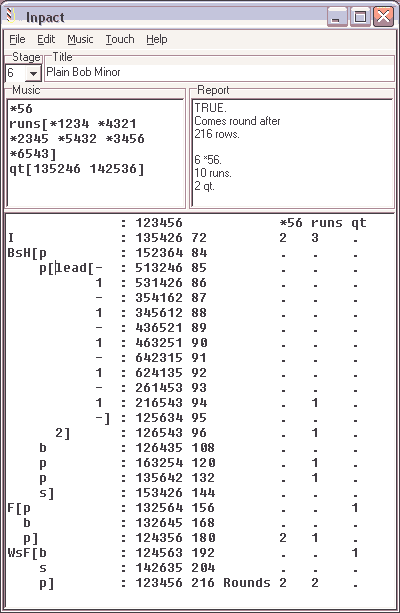
\includegraphics[width=0.4\textwidth]{inpact}
    \caption{Screenshot of Inpact}
\end{figure}



\pagebreak

\section{(TO REMOVE) Initial Design Decisions}

Now that we've taken a look at the state of the art, it's time to start making design decisions
about this project.  To do this, I will lay out my initial design and why I think it will satisfy
each of the design goals.

\br{}However, static web pages come with their own challenges.

\begin{enumerate}
    \item Storing persistent data in a cross-browser format is very challenging.  Cookies are an
        option but they are sent to the server with every HTTP request, making them unsuitable for
        storing large save states.
\end{enumerate}

\subsubsection{Using Cookies as Persistent State}

Fortunately for this project, there is some storage that web pages can use to store persistent data
without the user's input, and those are cookies.  Unfortunately, cookies are severely size limited
--- a web page can only expect to be able to save about 30 cookies per page, each of which can be at
most 4096 bytes, so we have 122,800 bytes in which to save all the persistent state we need.  In
reality, however, it's not a good idea to run too close to this limit because the page may have to
store other cookies and these shouldn't suddenly fail to save.

Saving just the current undo snapshot is fine, but I want to save the undo history which will
require a complicated serialisation/deserialisation algorithm.  I have chosen not to implement this
for the prototype, because I suspect that I will need to change the internal representation a lot
and doing so will break any serialised data.



\pagebreak

\section{Design}

The overall design of Jigsaw is an infinitely scrollable canvas which contains any number of
fragments in any location.  It is also designed to be used on a desktop with a 3-button mouse and
keyboard, and for maximal efficiency all common operations are triggered by keys on the left side of
the keyboard.  For consistency, all operations are applied at the location of the mouse cursor.

Overlaid on this canvas is a sidebar containing information which can't be represented using the
canvas interface.  This contains a lot of dense information, so all sections can be folded to hide
irrelevant information.

// List of keyboard shortcuts/operations

Fragments can be created or extended with \verb|a| (a single lead) or \verb|A| (a full course).

\begin{figure}
    \centering
    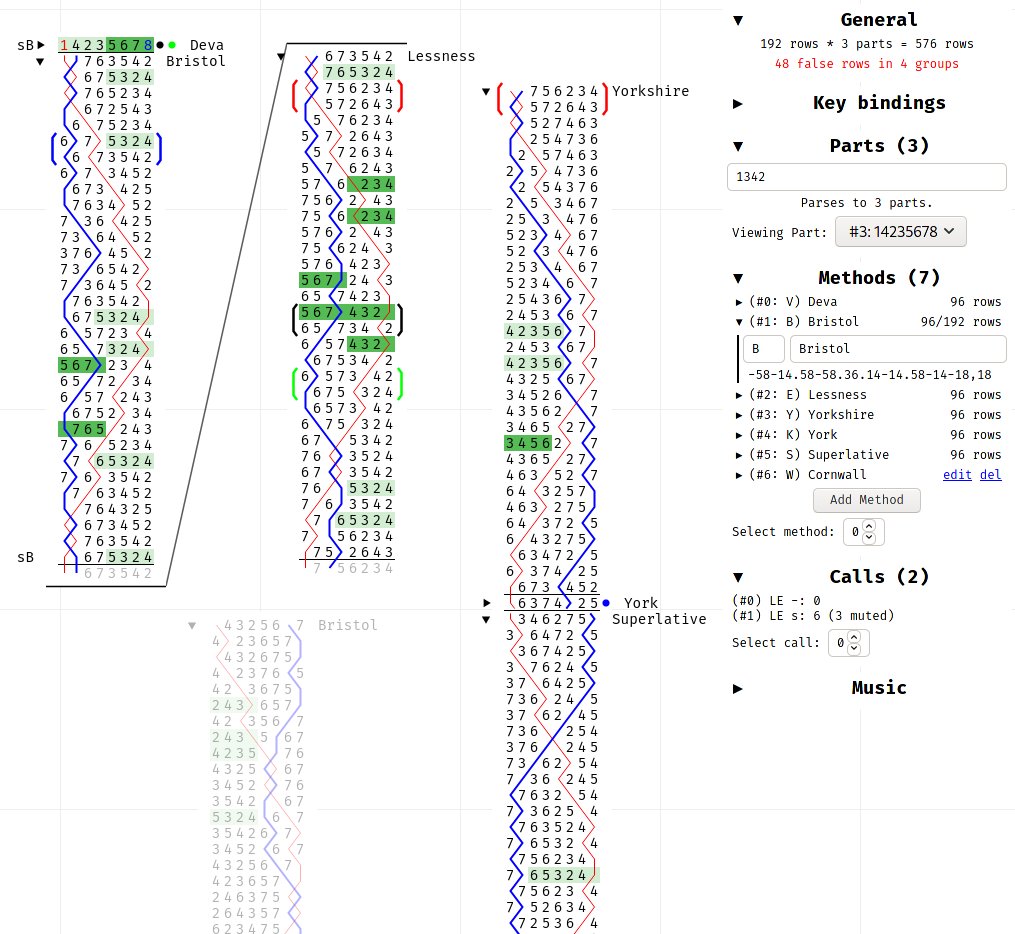
\includegraphics[width=0.8\textwidth]{current-screenshot-w-mute}
    \caption{Screenshot of Jigsaw, showing the folding UI and canvas display}\label{fig:cur-screenshot}
\end{figure}

\subsection{Music Highlighting}

When music appears in a composition, the bells causing the music are highlighted green, giving an
an obvious visual indication of where the music is.

Additionally, non-musical rows can generate music in other parts of the composition, and in this
case the music is `onion-skinned' --- the more parts contain music, the darker the colour.  In
Figure~\ref{fig:multi-part-music}, for example, \row{4328} in the \nth{1}{st} lead is highlighted quite
densely because it generates \row{5432}, \row{6543}, etc.\ in other parts.  However, \row{8761} in
the \nth{4}{th} lead is highlighted very lightly because it only creates \row{4321} in the \nth{2}{nd}
lead.

\begin{figure}
    \centering
    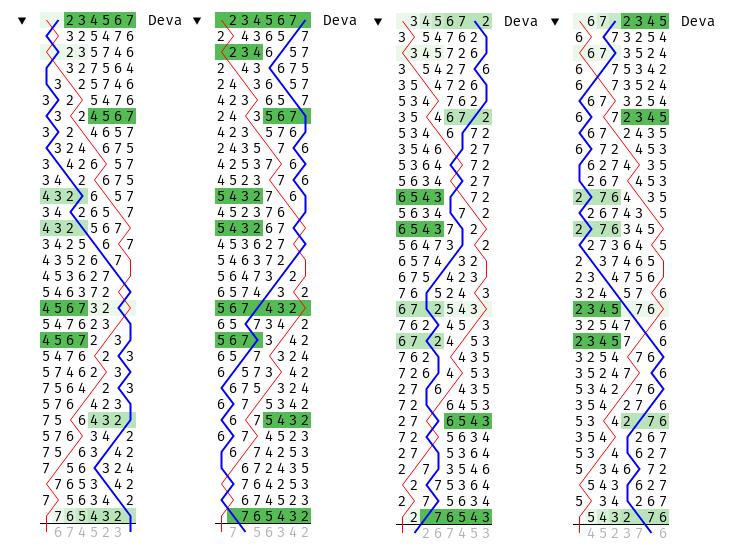
\includegraphics[width=0.6\textwidth]{multi-part-music-clean}
    \caption{The same lead in four different parts (rotating 2--8)}\label{fig:multi-part-music}
\end{figure}

\subsection{Falseness Display}

Falseness is visually communicated by marking groups of identical rows with the same coloured
brackets (see Figure~\ref{fig:falseness}).  As far as I know, this is the most efficient way of
visually communicating exact falseness.  The main drawbacks of this approach is that the number of
different groups can get very large causing Jigsaw to run out of easily differentiable colours.
Additionally, it is very reliant on colours which will likely be problematic for colour-blind
people.  A fix for this would be to add a switch to number the groups rather than just relying on
colour.

\begin{figure}
    \centering
    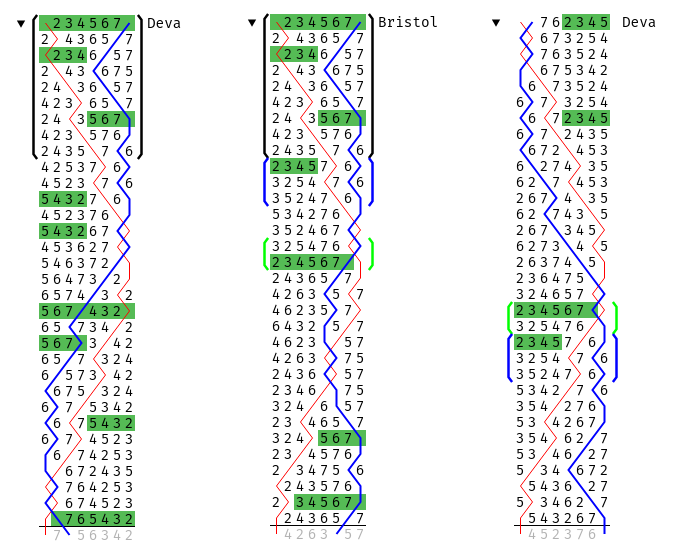
\includegraphics[width=0.5\textwidth]{falseness-clean}
    \caption{Leads which are false in 3 different ways}\label{fig:falseness}
\end{figure}

\subsection{Lead Folding}

To prevent the user from having to look at thousands of rows at the same time, Jigsaw allows leads
to be folded into a single row.  Jigsaw then converts falseness groups into dots next to the row
number (see Figure~\ref{fig:lead-folding}), and switches between lines and numbers for displaying
bells when necessary.

\begin{figure}
    \centering
    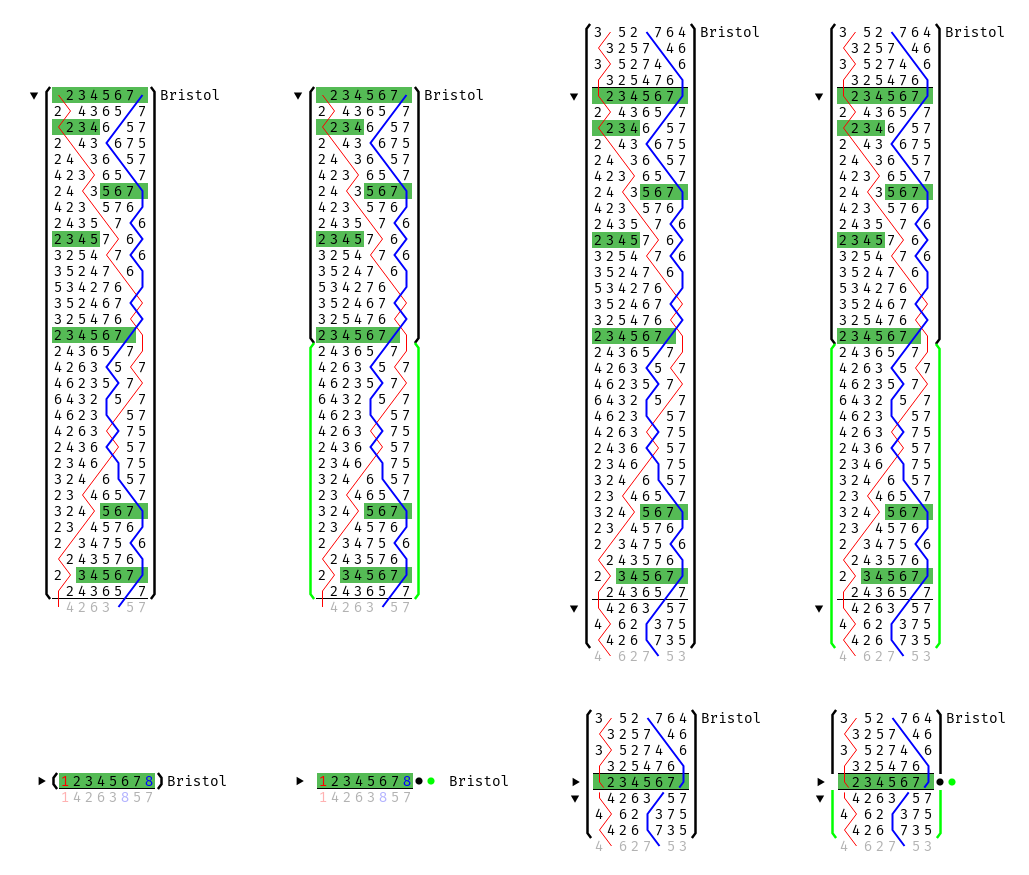
\includegraphics[width=0.78\textwidth]{folding-full}
    \caption{Unfolded (top) and folded (bottom) versions of the same lead.  Note the handling of
    falseness ranges and line segments.}\label{fig:lead-folding}
\end{figure}

\subsection{Linking Fragments}

Two fragments can be linked together if the leftover row of one is equal to the first row of the
other.  To represent this visually, Jigsaw draws a coloured line between the two (see
Figure~\ref{fig:linking}).  If multiple different sets of fragments link, then each group is
coloured separately (see Figure~\ref{fig:linking-insane}).

Hovering a line and pressing \verb|c| (for `connect') will join those fragments into one.  Note how
this operation doesn't change the rows contained in the composition.

\begin{figure}
    \centering
    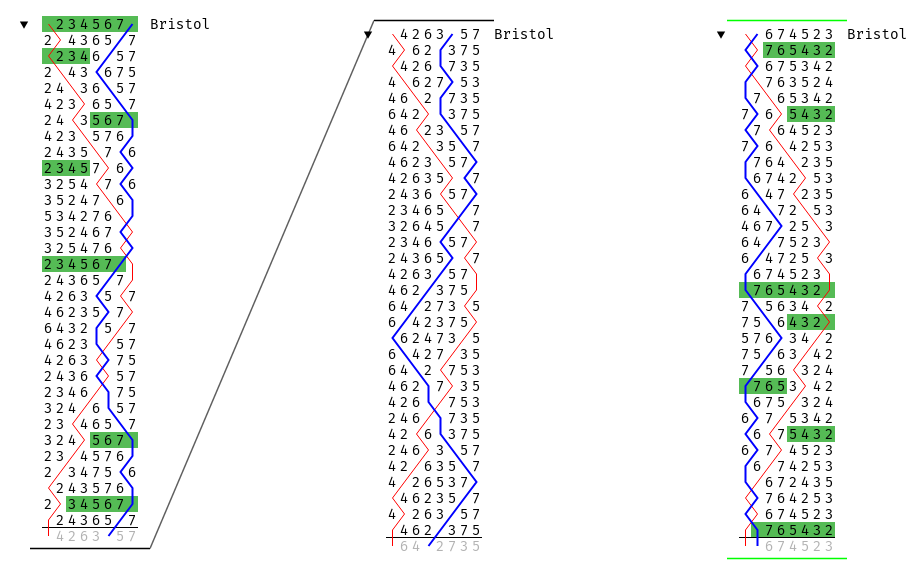
\includegraphics[width=0.8\textwidth]{linking-2}
    \caption{Two fragments which link together, and one that links to itself.}\label{fig:linking}
\end{figure}

\begin{figure}[h!]
    \centering
    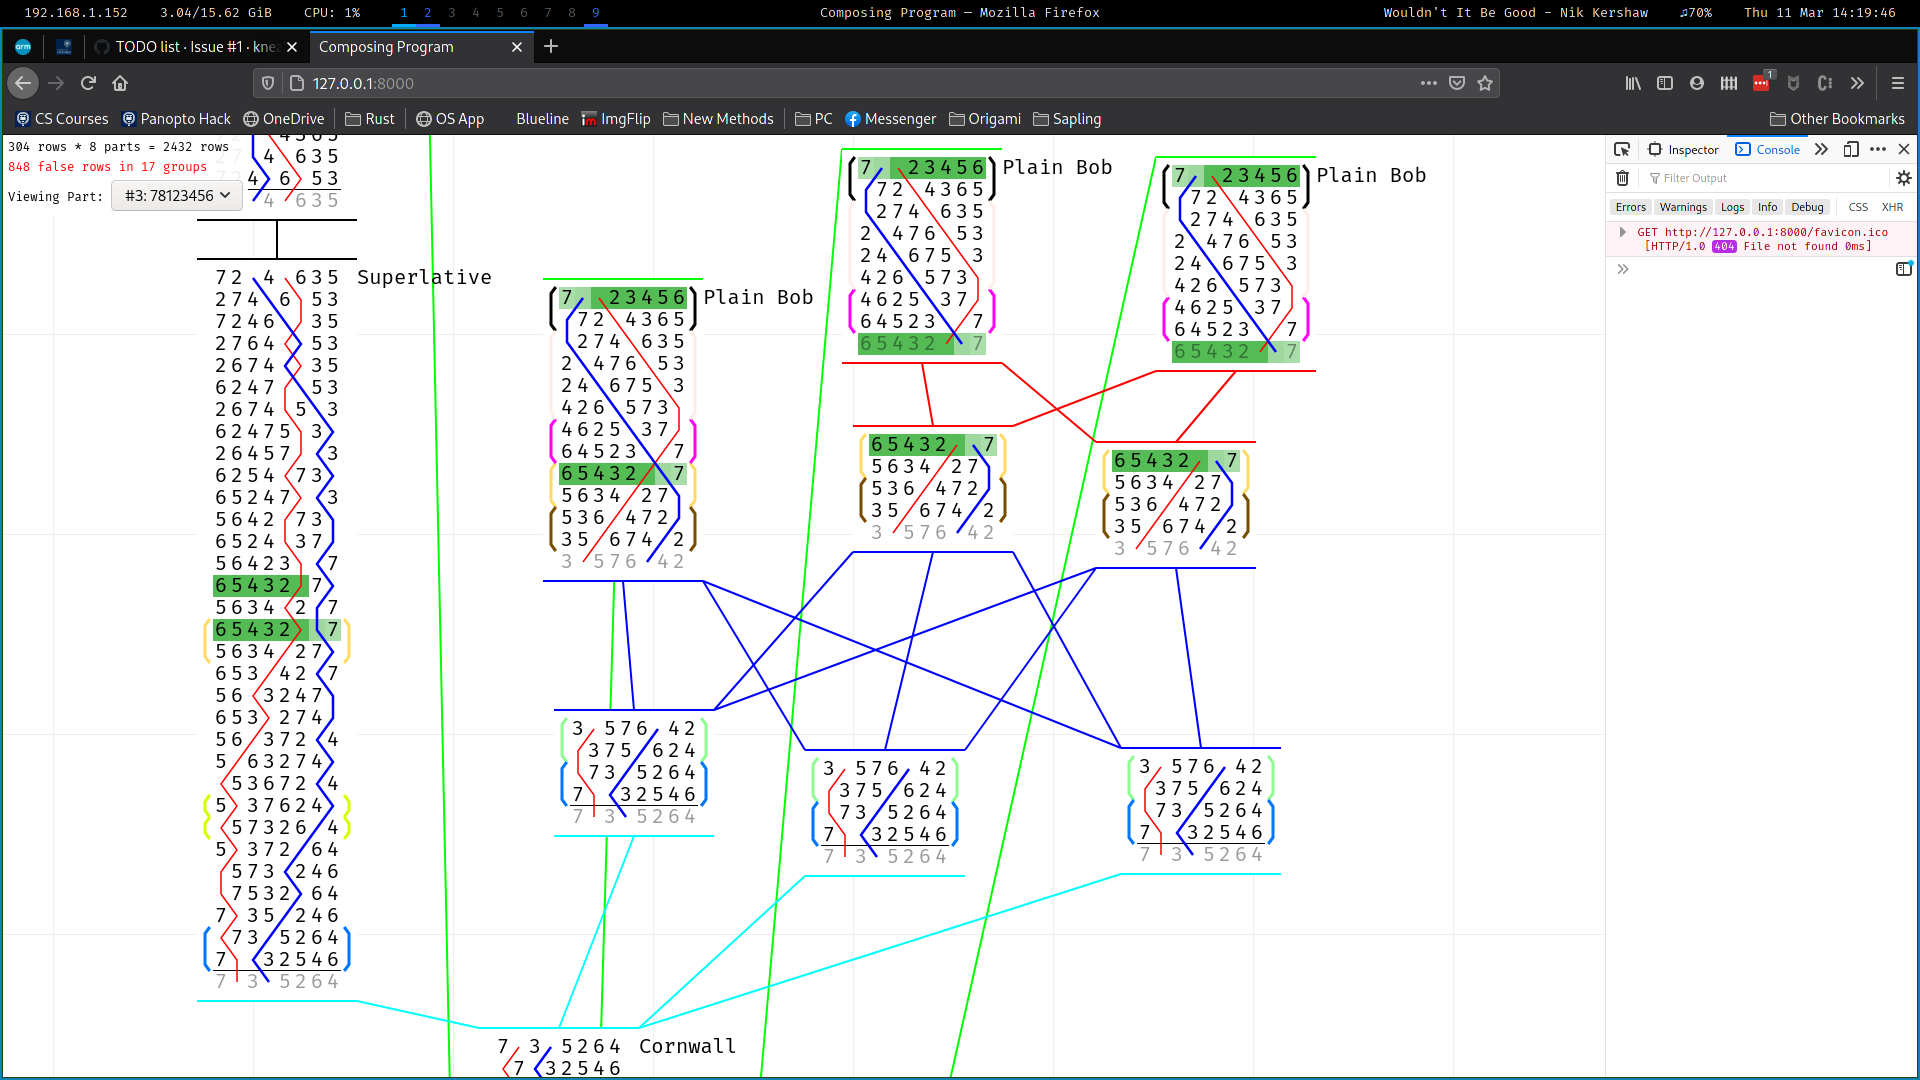
\includegraphics[width=\textwidth]{linking-insane}
    \caption{A lot of fragment links on one screen.}\label{fig:linking-insane}
\end{figure}

\section{Implementation}\label{sec:proj_arch}

The code for Jigsaw is split into 3 main parts: two Rust libraries which together form a `server'
and `client' in the form of a web GUI.\@  The Rust code is compiled to WebAssembly, and exports an
API which allows the JavaScript client to make changes to the internal `model' and then request a
JSON serialisation of the information to display to the user.  The whole application runs fully as a
single static web page, which is deployed automatically using GitHub pages.

This architecture plays to the strengths of both languages --- Rust provides fast and reliable data
manipulation whilst JavaScript, HTML and CSS provide a user-friendly cross-platform GUI.\@  The
binding and serialisation code is automatically generated at compile time using
\emph{wasm-bindgen}\footurl{https://github.com/rustwasm/wasm-bindgen} and
\emph{serde}\footurl{https://github.com/serde-rs/serde} to prevent human error.

\subsection{Utility Library}

Roughly half of the Rust code in the project is a cross-platform utility library for core datatypes
which are not specific to Jigsaw.  This provides safe and performant Rust datatypes for common
constructs related to change ringing (\verb|Row|, \verb|Bell|, \verb|Method|, \verb|Call|, etc.).
Its development and API design was motivated by Jigsaw but once its API is stable it will be
published to Rust's central package repository for general use.

The stable part of the API has good documentation and is well tested, and all datatypes only provide
public functions which preserve internal invariants and therefore obviate the need for unnecessary
checks.  It also provides `unsafe' versions of functions which remove runtime checks but in rely on
their caller to uphold the invariants.  Therefore, no undefined behaviour is possible if the user
only writes `safe' code.

Despite have no stable API, I have already built other projects on it.  In its own right, this
library is a valuable product of this project.

\subsection{Model View Presenter}

Over the course of the project, the architecture of the application settled naturally into the
`Model-View-Presenter'
model\footurl{https://en.wikipedia.org/wiki/Model\%E2\%80\%93view\%E2\%80\%93presenter}.  The View
is the web code in \verb|www/| (written in JavaScript/HTML/CSS) while the \verb|jigsaw| library
holds both the Model and the Presenter.

\subsection{Specification vs Derived State}

The code in the jigsaw library differentiates between the unique specification of a composition
(the \verb|Spec| type) and the information required to display it to the user (the
\verb|DerivedState| type).  The \verb|DerivedState| contains additional data like the music
locations, falseness and other annotations.  That is completely specified by the contents of the
current \verb|Spec|, so every change to the \verb|Spec| must also cause the \verb|DerivedState| to
be updated before the changes can be displayed to the user.

In terms of Model-View-Presenter, the \verb|Spec| type is the Model whereas the \verb|DerivedState|
is the data sent from the Presenter to the View.

The undo history is simply a list of \verb|Spec| types along with an index.  The internal data of
\verb|Spec|s is always stored through immutable reference counted pointers, which prevents
unnecessary cloning without data leaks or mutation of shared memory.

\subsection{Architectural Invariants}

This architecture of Model-View-Presenter and immutable history requires a number of invariants to
be upheld while the application is running.

Firstly, there are two separate copies of \verb|DerivedState| which must be kept in sync.
Additionally, the \verb|DerivedState| is entirely specified by the \verb|Spec| currently being
displayed so both copies must be kept in sync with that too (because the \verb|DerivedState| is
where JavaScript gets its display data from).  In two cases this invariant is temporarily broken
(while dragging fragments and panning the viewport) for performance reasons.  Upholding the
invariant in these cases would (currently) cause the entire \verb|DerivedState| to be regenerated
every time the user moves the mouse, creating a completely unnecessary drop in performance.

Secondly, the JavaScript code and the \verb|Spec| datatypes should be be completely decoupled, and
should only communicate through the \verb|Comp| singleton.  This constraint is inherited from the
Model-View-Presenter model (where the Model and View can only communicate through the Presenter).

\subsection{Data Flow}

These invariants enforce a very specific data flow whenever the user changes the composition
(summarised in Figure~\ref{fig:app_data_flow}).  The user's input events are all captured by
JavaScript, which calls a corresponding function in \verb|Comp|'s API.\@ The \verb|Comp| singleton
then clones the current \verb|Spec|, performs the required modifications and then pushes it onto the
history stack.  Next, \verb|Comp| rebuilds its copy of \verb|DerivedState| to reflect the changes in
the \verb|Spec| (thus upholding the invariants).  At this point, the WebAssembly function returns
control to JavaScript which immediately calls \verb|Comp::ser_derived_state| which returns a JSON
string with which to overwrite the \verb|derived_state| variable.

\begin{figure}
    \centering
    \begin{BVerbatim}
        JS          |        Rust
--------------------+--------------------
     User input     |
         |          |
         v      API Call
       Event -------------> Comp API
         |          |          |
         |          |          v
         |          |      Clone Spec
         | undo/    |          |
         | redo     |          v
         |          |    Modify new Spec
         |          |          |
         |          |          v
         \-------------> Update History
             API Call          |
                    |          v
         /------------ Rebuild DerivedState
         |   return |
         |          |
 sync_derived_state |
         \-------------> ser_derived_state
             API Call          |
                    |       (serde)
                    |          v
   JSON String <--------- JSON String
        |        return
  (deserialise)     |
        v           |
  derived_state     |
        |           |
        v           |
     repaint        |
    \end{BVerbatim}
    \caption{The data flow of user's changes}\label{fig:app_data_flow}
\end{figure}



\pagebreak

\section{Failed Design Decisions}

\subsection{Facebook Poll}

(Dec 3, Poll linked
below\footurl{https://www.facebook.com/groups/601658156640471/permalink/2097786800360925})

Having lain down a rough initial design, I wanted feedback from other composers to determine if it
would be widely useful.  I am self-taught in composing, and it's entirely possible that I have a
completely non-standard workflow.

To achieve this, I posted an open question on a Facebook group that I know is frequented by other
composers asking (in general terms) what their composing workflow was.  I got a good number of
responses (64 comments in total), and there was a surprising variety in approaches.  Some people
generate compositions entirely through computer search (which is out of scope for this project) but
most composers compose by hand.  Of these, nearly everyone said that they build up compositions from
small pieces and agreed that my design would be interesting and potentially useful.  (N.B. Possibly
put something here about coursing orders/course heads, but I'm not sure if it's relevant).

\subsection{Talk with Anders Holroyd}

TODO

\subsection{Rows vs Permutations}

When building the utility library, I initially thought that the concept of rows and permutations
were different enough to warrant separate data types.  My thinking was that a \verb|Row| is a
sequence of \verb|Bell|s (plus some additional invariants), and a permutation can be thought of as a
function of type \verb|[a] -> [a]| which can permute sequences of any type.  Mathematically this
feels like an elegant separation, but using the library in ernest made me realise that the
\verb|Perm| doesn't pull its weight given its large overlap with the \verb|Row| type.  I would
almost always use \verb|Perm| only as an intermediate step to use one \verb|Row| to permute another.
Therefore, a few months into the project the operations of the \verb|Perm| structure was merged into
\verb|Row|.

\subsection{Passing Data Between Rust and JavaScript}

Even with the \emph{wasm-bindgen} generated code, the types that can be sent
over the language interface is limited to flat structures with no references.  This is unfortunate,
since the internal data structures have 3 layers of references.

Initially, I didn't want JavaScript and Rust to hold their own copies of the same data, since there
would be two potentially divergent sources of the truth.  Also, I wanted to limit the complexity of
the JavaScript code (due to its inferior performance and maintainability) so it made sense for Rust
to handle all the state and then expose a simple API to JavaScript to read or modify this data.

The modification part of the API provides one function per operation on the composition, which
enforces a separation of concerns because JavaScript has no knowledge of how Rust chooses to
implement these functions.  This worked excellently and I had no issues with it.

In order to work round the inherent issues of WebAssembly, the initial data read API was a flat set
of getter functions, looking like Figure~\ref{fig:initial_api}.  This worked fine for a while but as
the complexity of the datatypes grew, the number of exported functions exploded and refactoring the
API became an unnecessary challenge.  Also, every WebAssembly function call takes a non-trivial
amount of time and this flat API encourages huge numbers of calls each frame which started causing
performance issues.

\begin{figure}
    \begin{verbatim}
/// Get the number of fragments
fn get_num_frags() -> usize { ... }

/// Get the number of rows in the fragment at a given index
fn get_frag_length(frag_index: usize) -> usize { ... }

/// Get the bell at a given location
fn get_row(
    frag_index: usize,
    row_index: usize,
    bell_index: usize
) -> Bell { ... }
    \end{verbatim}
    \caption{Initial getter API design}\label{fig:initial_api}
\end{figure}

It's also worth noting that the data being read only changes when the user edits the composition,
not every frame.  Also, we are rebuilding the \verb|DerivedState| anyway every time the user edits
the composition, and this structure holds all the data required for JavaScript to render the
composition (see Section~\ref{sec:proj_arch} for the final architecture).  Therefore, I tried
passing the entire \verb|DerivedState| as a JSON string for JavaScript to deserialise and store.
Serialisation in Rust is extremely easy due to
\emph{serde}\footurl{https://github.com/serde-rs/serde}, a library which generates
(de)serialisation code for any data type at compile-time.  This turned out to work really well ---
almost no WebAssembly calls are made during each frame, the API size and complexity is significantly
reduced and long-term divergence is impossible because JavaScript overwrites its copy of the
\verb|DerivedState|.  Also, refactoring the data is usually a simple matter of find/replace of the
JavaScript code.  

\subsection{Mute/Solo}

The system for muting/soloing fragments went through several iterations.  Mute/solo is most common
in music production applications, where it's often useful to listen to only some sounds in
isolation.

The dominant design gives each item 3 states: \emph{normal}, \emph{muted} or \emph{soloed}.  If any
items are soloed, then all the non-soloed items are silent, otherwise only muted items are silent.
However, visual feedback for all 3 states is required because normal and muted are indistinguishable
when items are soloed.  This didn't fit with the minimalist design aesthetic of Jigsaw, so I used a
strategy inspired by the music software FL Studio\footurl{https://www.image-line.com/}.

In this design, each item has only two states: \emph{normal} or \emph{muted}, visually indicated by
greying out muted fragments (see Figure~\ref{fig:frag-mute}).  There are still two operations:
`mute' (key: \verb|s|) and `solo' (key: \verb|S|).  Mute simply toggles the state.  If the fragment
is the only unmuted fragment, then solo unmutes everything, otherwise it mutes everything except the
hovered fragment.

\begin{figure}
    \centering
    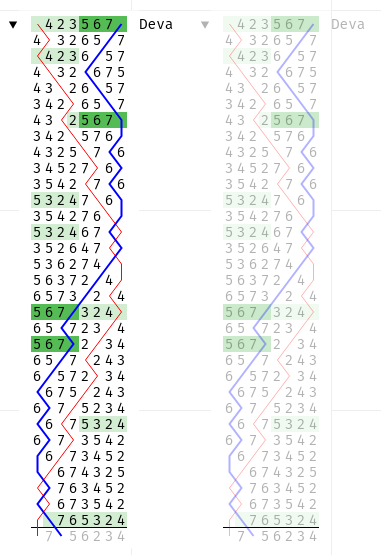
\includegraphics[width=0.3\textwidth]{muted-frag}
    \caption{Normal vs muted fragments}\label{fig:frag-mute}
\end{figure}


\subsection{Block Structure}

TODO

\subsection{Line Rendering}\label{sec:line-rendering}

TODO

\subsection{Non-Group Multi-parts}

TODO

\subsection{Final Stats}

As of writing this report, the project clocks in at 275 commits, 5,736 source lines of code
(including 4,233 of Rust, 1,033 of JavaScript, 240 of HTML, 114 of CSS and 85 of Python for the
build script).



\pagebreak

\section{Conclusion}

This project has two major products: the application itself (Jigsaw) and the reusable utility
library on which Jigsaw is built.

I think that Jigsaw is a successful prototype and I will likely continue building it into a
feature-complete application.  I demonstrated it to several other composers who all thought it
looked very promising.  It has a number of small rough edges which would make the current iteration
difficult to use in production, but do not detract from its value as a prototype.

In order to decide on the success of the project, I will rank it against the design goals set out in
Section~\ref{sec:design-goals}.

\subsection{Ease of Use \& Visual}

Firstly, building Jigsaw as a single static page means it requires no installation to use.  The
design of an infinite canvas plus a folding sidebar feels very intuitive to use.

A large amount of effort went into making sure that GUI is visually crisp and responsive.  This
goes as far as rounding all coordinates to the nearest pixel to prevent fuzzy boundaries
(screenshot?), as well as doing the same for line rendering --- see
Section~\ref{sec:line-rendering}.  This attention to detail makes the experience of using Jigsaw
feel very smooth and polished.

All actions are currently bound to keyboard shortcuts which means that editing compositions quickly
becomes muscle memory for experienced users, but feels unintuitive to beginners since at any point
in time there's no indicator of what actions are available.  If I had more time, I would add a
contextual right-click menu to fix this problem (it could even show the key bindings to help
beginners learn them).

\subsection{Completeness}

Jigsaw's internal representation is complete, but the current user interface is not.  In other
words, Jigsaw is internally able to represent a strict superset of compositions which are considered
change ringing, but the prototype GUI means that the user is unable to express some very obscure
states which are technically considered change ringing.  For perhaps 99\% of use cases, Jigsaw's
user interface is complete enough that most users would not notice.

\subsection{Incremental}

Jigsaw is completely built around being incremental.  It also does its best to preserve `continuity'
of operations --- that is, a small operation should cause a small change to the composition's rows.
Some operations like splitting and joining fragments only change the structure of the composition,
and not the output rows.

\subsection{Instant}

Due to the internal architecture, the composition is always fully annotated.  Whenever the user
causes an update, the entire state of the display is recalculated then cached for repainting.
Therefore, it simply isn't possible for any part of the changes to lag behind because the full UI
state is simultaneously recalculated after every change.

This does, however, mean that Jigsaw is extremely dependent on the efficiency of this update
pipeline.  Luckily, Rust and WebAssembly seem to be working extremely well here since the pipeline
is fast enough to reliably feel instant, even for extremely large compositions.  I haven't done any
specific optimisations, but I have also been mindful of high-level performance when writing the code
--- the algorithms are all $O(n \log n)$ in the number of bells in the composition, although the
link detection is $O(n^2)$ in the number of fragments.

Whilst stress testing Jigsaw, I discovered that this delay becomes noticeable at around 35,000
$\times$ 8 = 280,000 bells (see Figure~\ref{fig:stress-test}).  Since at least 99.9\% of
compositions have at most 10,000 rows each of 16 bells (making 160,000 bells total) I think that the
performance is perfectly adequate.

The longest piece of ringing ever rung contains 72,000 $\times$ 6 = 432,000 bells, which would cause
the current implementation some consternation.  However, there is plenty of low hanging fruit left
to optimise --- there is no caching or re-use of allocations so the code causes huge numbers of
allocations during each pipeline run.

Lastly, \verb|bell_frame| contains the \verb|SimdRow| type which uses SIMD instructions
(specifically \verb|pshufb|) to perform row permutations in a single clock cycle, which usually
increases performance by at least an order of magnitude.  However, SIMD support in WebAssembly is
not mainstream yet so Jigsaw can't take advantage of this.

\begin{figure}
    \centering
    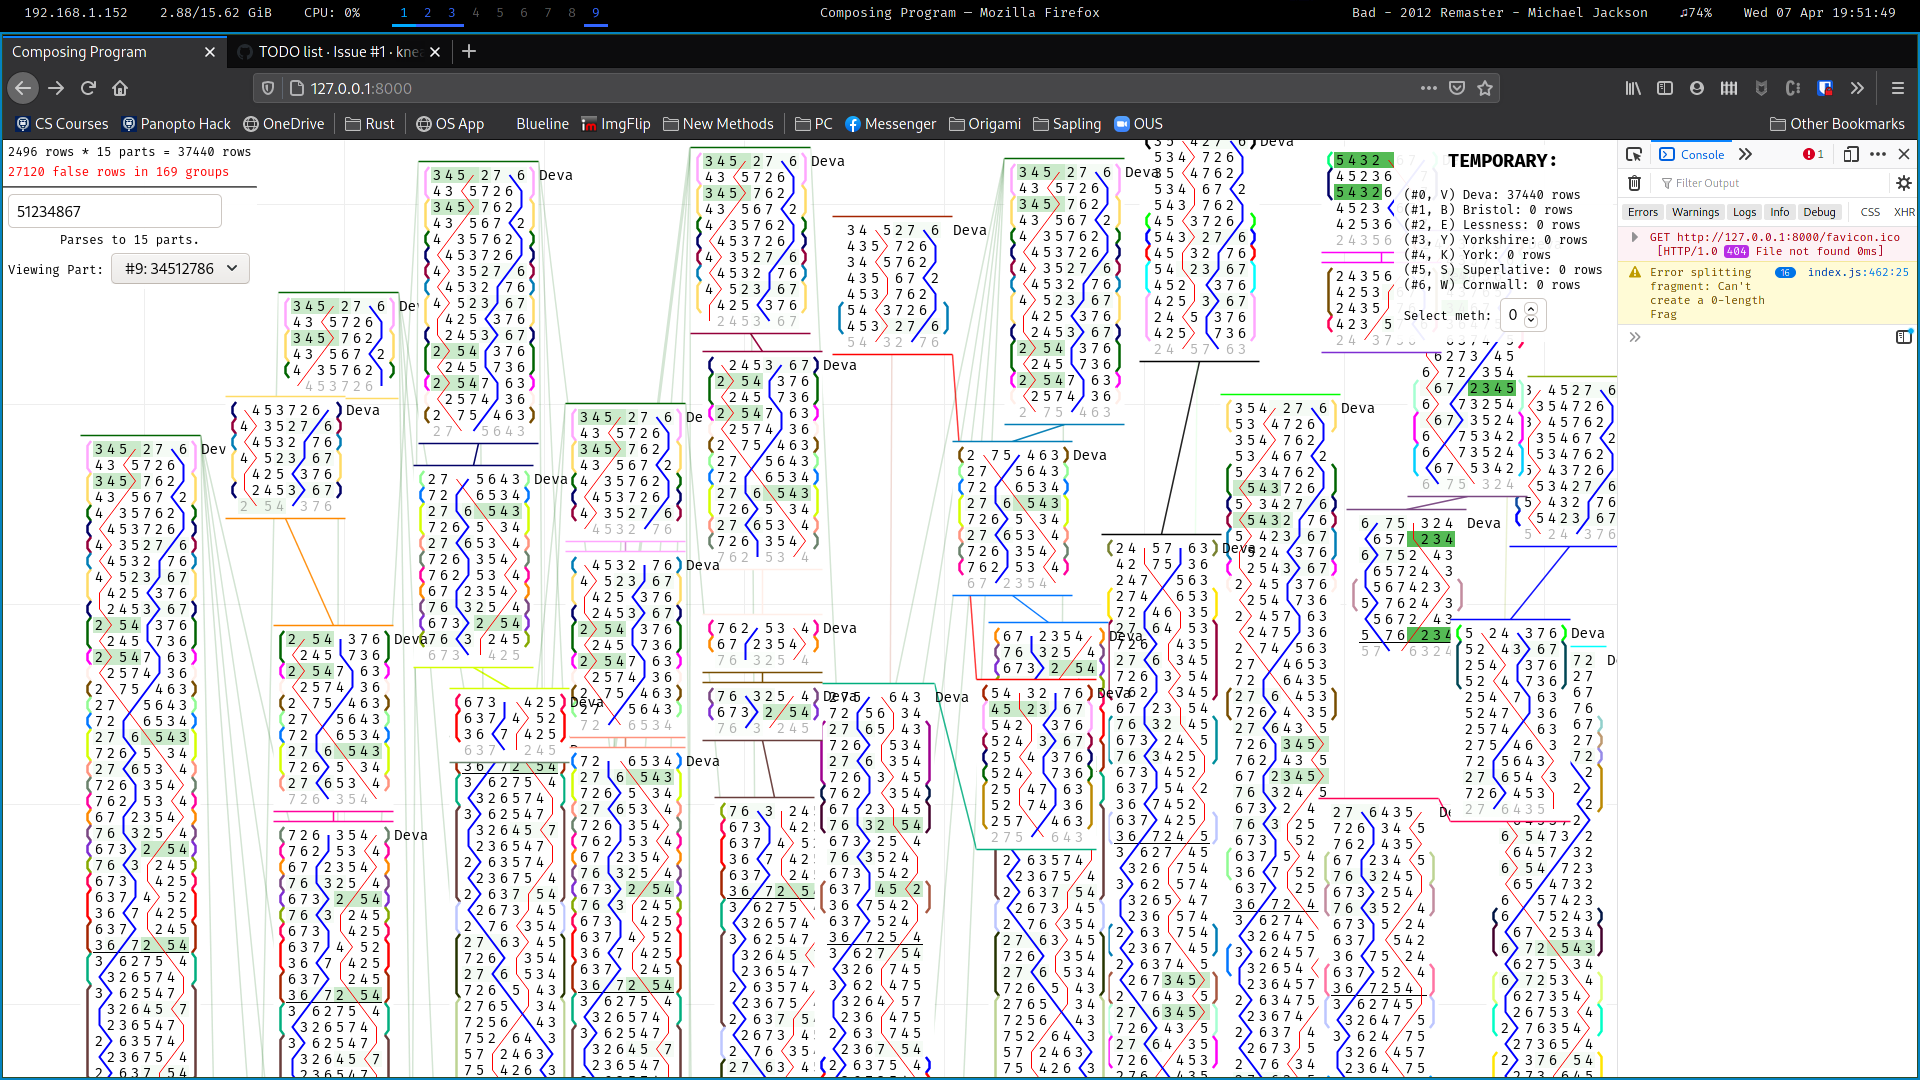
\includegraphics[width=\textwidth]{stress-test}
    \caption{Stress testing Jigsaw (the GUI has since changed, but the pipeline has
    not).}\label{fig:stress-test}
\end{figure}



\pagebreak

\section{Glossary of Change Ringing Terms}

\paragraph{Stage:} The number of bells which the composition uses.  This is not necessarily the
number of bells used to ring a given composition, but for the purposes of this project the
distinction is not relevant.

\paragraph{Row:} A sequence of bells which forms a permutation.  Rows are the fundamental building
blocks of compositions.  The words `change' and `row' are often used interchangeably (hence the name
`Change Ringing'), but to avoid confusion I will always use `row' in this report.

\paragraph{Composition:} An ordered sequence of rows which tell ringers in which order the bells
should be rung.

\paragraph{Truth:} For the purposes of this project, a composition is \emph{`true'} if all the rows
are unique, otherwise it is \emph{`false'}.  This is the single most important property of a
composition, since any performance of a `false' composition is considered invalid.

\paragraph{Method:} A short, usually symmetrical, pattern that is repeated throughout a composition
with small and well-defined modifications (known as `calls').  This is the key to how human ringers
can ring over 5000 rows worth of composition without any memory aid --- in reality, they memorise
the method(s) and one `conductor' memorises the pattern of calls and calls them in the right places
for the other ringers to take effect.  It is usually the job of the composer to make sure that the
call sequence is predictable and easy to memorise.

\paragraph{Lead:} A single instance of the repeating pattern of a method.

\end{document}
